\section{Diseño}

\subsection{planteamiento de circuito}
Como se menciono anteriormente, utilizando el modulo de matriz de leds MD\_7219.
Utilizando el microcontrolador Arduino Uno, utilizando las entradas digitales se debe 
colocar que lean los botones, siendo este uno rojo y azul. El botón rojo debe hacer que la matriz 
incremente en uno el contador que se lleva hasta llegar a F, si se pasa de F este debe volver a 0. El botón
azul debe hacer que la cuenta disminuya por cada toque hasta llegar a 0, si este se presiona nuevamente se debe
regresar a F. Teniendo el anterior planteamiento y conectando el modulo directo a la placa, con la alimentación
de $\SI{5}{\volt}$ y a tierra, se tiene el siguiente diagrama:
\begin{figure}[h!]
    \centering
    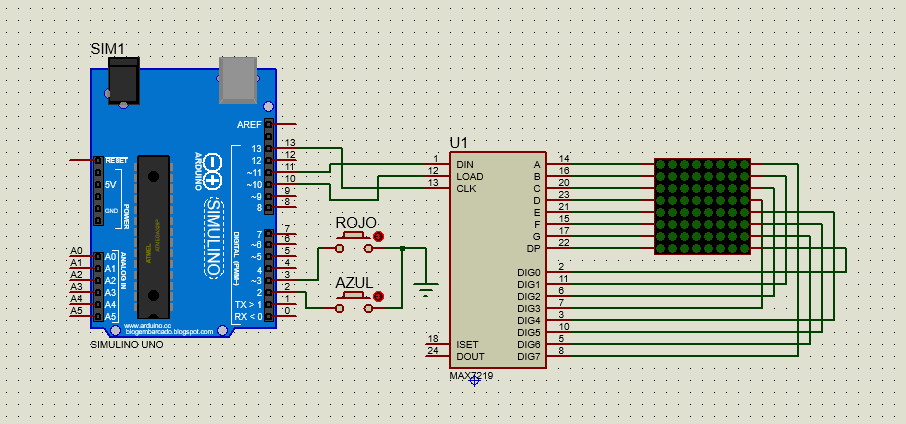
\includegraphics[width=0.8\textwidth]{Diagramas/Diagrama.png}
    \caption{Diagrama de conexión}
    \label{fig:conexion}
\end{figure}

Ahora bien, ya que el modulo no existe en el simulador, se construyo utilizando el circuito integrado y una matriz de leds
entregadas por el programa. Igualmente, se observan ambos botones conectados a tierra. Estos botones, están en configuración
de pull up, osea que los pines están energizados en $\SI{5}{\volt}$ mediante una resistencia de pull up, entregando el valor HIGH,
si se presiona el botón, este pasa a LOW, teniendo asi las entradas digitales de nuestro montaje. Para la salida de nuestro circuito 
se tiene la matriz construido, asi esta se tiene que conectar a un voltaje de alimentación y a tierra, pero en proteus no se puede realizar esto, 
pero teniendo considerado esto para la implementación del circuito.

\subsection{Desarrollo del código}
Para el desarrollo del código que se implementa en el Arduino Uno, se utilizo la biblioteca \texttt{MD\_MAX72xx}